\documentclass[border=4pt]{standalone}
\usepackage{tikz}
\usetikzlibrary{calc,positioning,shapes.geometric}
\begin{document}
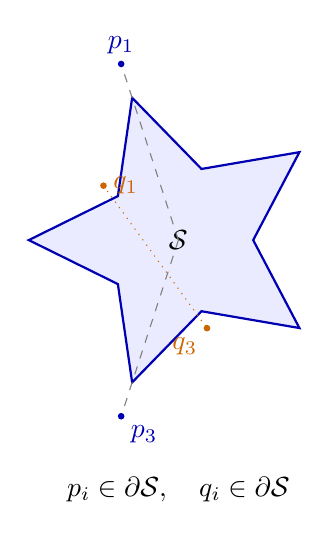
\begin{tikzpicture}
  \node[star,star points=5,star point ratio=2,star rotate=18,
    minimum size=38mm,outer sep=2mm,draw=blue!70!black,
    thick,fill=blue!8] (S) {$\mathcal S$};

  \draw[dashed,gray] (S.center) -- (S.outer point 1);
  \draw[dashed,gray] (S.center) -- (S.outer point 3);
  \draw[dotted,orange!80!black] (S.inner point 1) -- (S.inner point 3);
  \fill[blue!70!black] (S.outer point 1) circle (1.2pt)
    node[above] {$p_1$};
  \fill[blue!70!black] (S.outer point 3) circle (1.2pt)
    node[below right] {$p_3$};
  \fill[orange!80!black] (S.inner point 1) circle (1.2pt)
    node[right] {$q_1$};
  \fill[orange!80!black] (S.inner point 3) circle (1.2pt)
    node[below left] {$q_3$};
  \node[below=14mm of S] {$p_i\in\partial\mathcal S,\quad q_i\in\partial\mathcal S$};
\end{tikzpicture}
\end{document}
